\chapter{Solution}

\section{A* Algorithm}

\paragraph{} ~\\
A* uses a best-first search and finds a least-cost path from a given initial node to one goal node (out of one or more possible goals). As A* traverses the graph, it follows a path of the lowest expected total cost or distance, keeping a sorted priority queue of alternate path segments along the way.
\paragraph{} ~\\
It uses a knowledge-plus-heuristic cost function of node x (usually denoted f(x)) to determine the order in which the search visits nodes in the tree. The cost function is a sum of two functions:


\begin{itemize}
\item{The past path-cost function, which is the known distance from the starting node to the current node x (usually denoted g(x))}
\item{A future path-cost function, which is an admissible "heuristic estimate" of the distance from x to the goal (usually denoted h(x)).}
\end{itemize}

\subsection{A* Algorithm Process}
\paragraph{} ~\\
The h(x) part of the f(x) function must be an admissible heuristic; that is, it must not overestimate the distance to the goal. Thus, for an application like routing, h(x) might represent the straight-line distance to the goal, since that is physically the smallest possible distance between any two points or nodes. 

\paragraph{} ~\\
Like all informed search algorithms, it first searches the routes that appear to be most likely to lead towards the goal. What sets A* apart from a greedy best-first search is that it also takes the distance already traveled into account; the g(x) part of the heuristic is the cost from the starting point, not simply the local cost from the previously expanded node.

\paragraph{} ~\\
Starting with the initial node, it maintains a priority queue of nodes to be traversed, known as the open set or fringe. The lower f(x) for a given node x, the higher its priority. At each step of the algorithm, the node with the lowest f(x) value is removed from the queue, the f and g values of its neighbors are updated accordingly, and these neighbors are added to the queue. The algorithm continues until a goal node has a lower f value than any node in the queue (or until the queue is empty). (Goal nodes may be passed over multiple times if there remain other nodes with lower f values, as they may lead to a shorter path to a goal.) The f value of the goal is then the length of the shortest path, since h at the goal is zero in an admissible heuristic.
\paragraph{} ~\\
The algorithm described so far gives us only the length of the shortest path. To find the actual sequence of steps, the algorithm can be easily revised so that each node on the path keeps track of its predecessor. After this algorithm is run, the ending node will point to its predecessor, and so on, until some node's predecessor is the start node.

\begin{figure}[H]
    \centering
    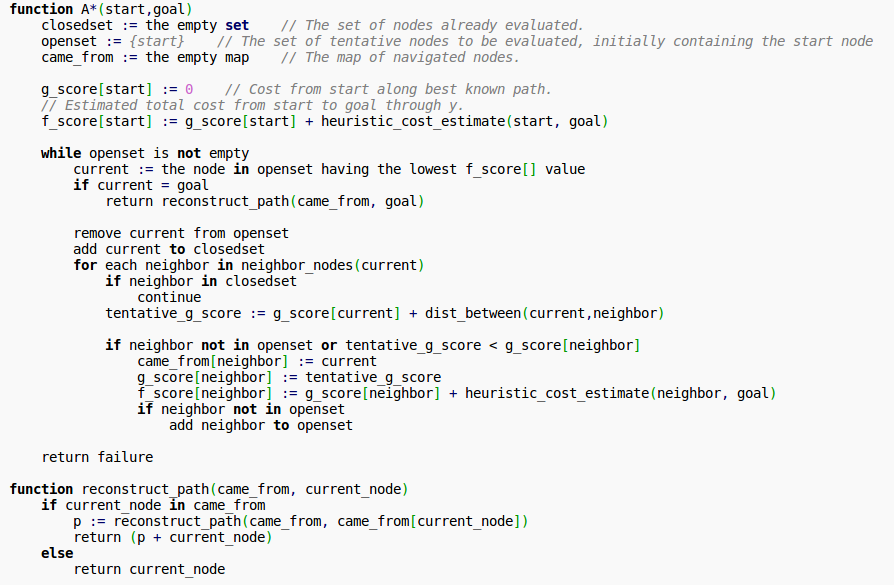
\includegraphics[width=.8\textwidth]{images/astar_pseudocode.png}
    \caption{A* Algorithm Pseudocode}
    \label{fig:astar_pseudocode}
\end{figure}

\section{A* for path finding in ITESM Parking Lot}
\paragraph{} ~\\
The ITESM parking lot has more than 3000 parking lots that are distributed near to common areas like Library, High School, Administrative offices, Conferences Center, etc.
In order to represent the parking lot distribution as a conected graph, it's required to separate parking sections based on the location and the nearest buildings areas 
they are set.
As we show in Figure 3.2, here's how each node type is being configured:
\begin{itemize}
\item{Parking of Lot Start}
\subitem{List of Destinations with (Name and Estimated Distance h(x))}
\subitem{Node Type}
\item{Section}
\subitem{List of Destinations with (Name and Estimated Distance h(x))}
\subitem{Calculated path cost from start to section g(x)}
\subitem{Neighbors (Section or Slots)}
\subitem{Node Type}
\item{Parking Slot}
\subitem{List of Destinations with (Name and Estimated Distance h(x))}
\subitem{Calculated path cost from start to section g(x)}
\subitem{Neighbors (Slots)}
\subitem{Node Type}
\item{Destinations}
\subitem{The final visited node(slot) should be conected to the final destination (Example: Conferences Center)}
\end{itemize}

\begin{figure}[H]
    \centering
    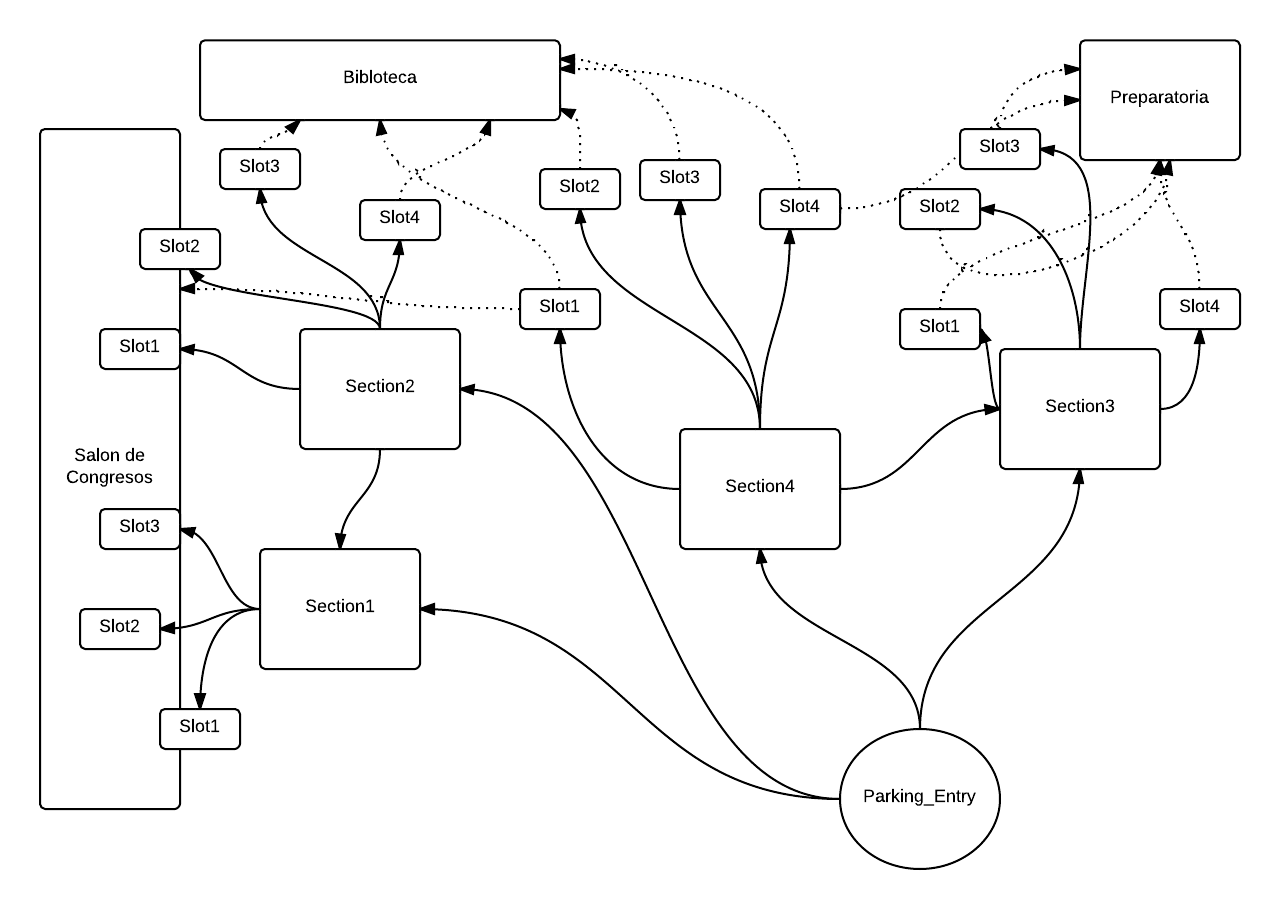
\includegraphics[width=1\textwidth]{images/parking_lot_diagram.png}
    \caption{Example of Graph used for representing Parking Lot sections/slots conections}
    \label{fig:parking_lot_diagram}
\end{figure}

\paragraph{} ~\\
Once we have our graph representation we are able to perform slot searches. It's really important to keep the type of Node when visiting it in the A* Algorithm. The type 
of Node will be saying if it's an end node or if it cannot be a final node. For example, a Section Node, cannot be the end because it's a forbidden area to park, you 
need to park in the slot-type nodes.

\section{Source Code Implementation}

\subsection{Node class}
\begin{figure}[H]
    \centering
    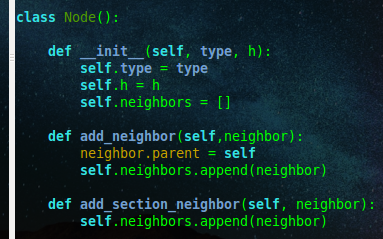
\includegraphics[width=.7\textwidth]{images/node_class.png}
    \caption{Node Class Definition}
    \label{fig:node_class}
\end{figure}

\subsection{Graph Builder}
\begin{figure}[H]
    \centering
    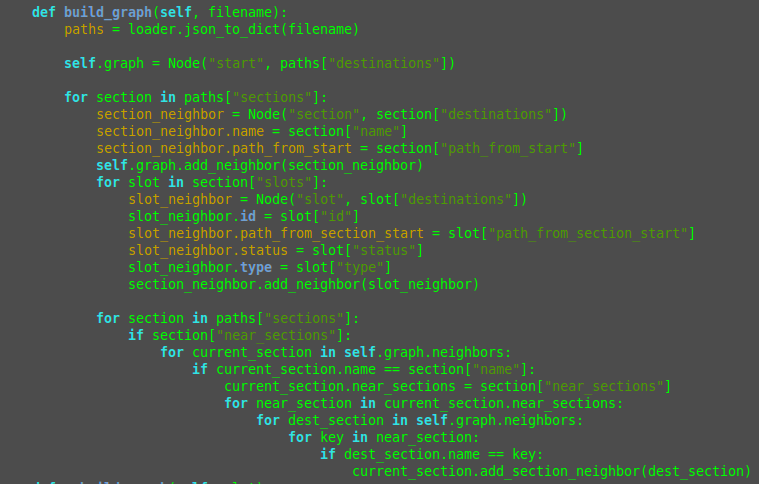
\includegraphics[width=1\textwidth]{images/graph_builder.png}
    \caption{Graph Builder Function}
    \label{fig:graph_builder}
\end{figure}

\subsection{f(x) = g(x) + h(x) Calculation}
\begin{figure}[H]
    \centering
    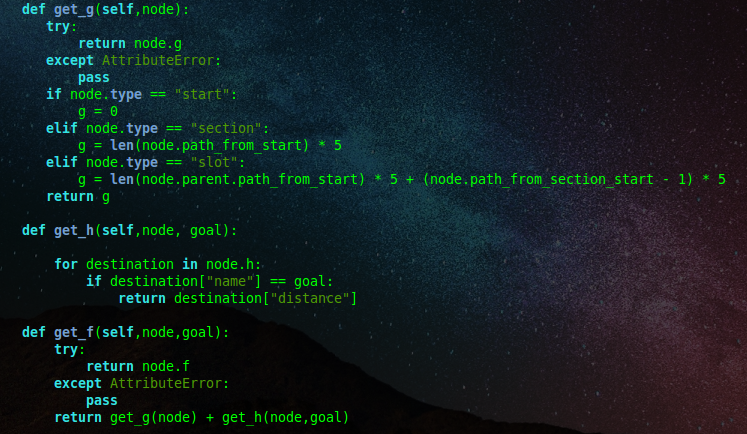
\includegraphics[width=.9\textwidth]{images/f_g_h.png}
    \caption{Functions to calculate f(x) = g(x) + h(h)}
    \label{fig:f_g_h}
\end{figure}

\subsection{A Star Algorithm}
\begin{figure}[H]
    \centering
    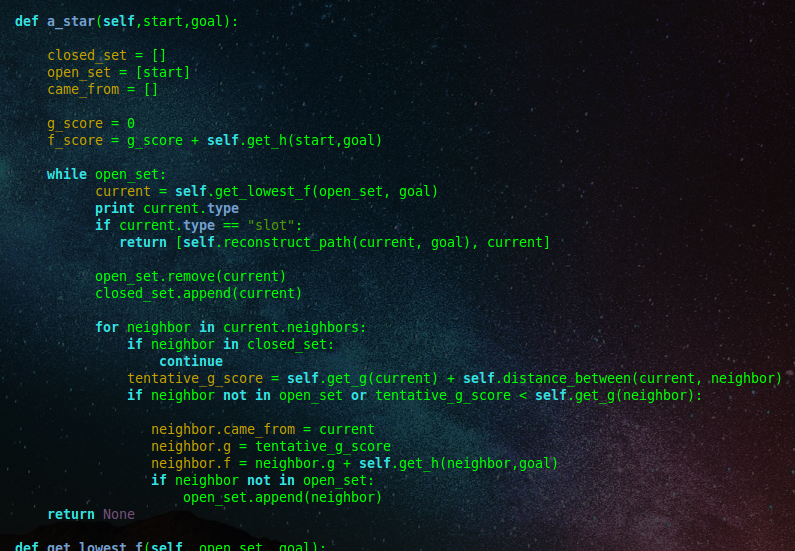
\includegraphics[width=.9\textwidth]{images/a_star.png}
    \caption{A* Algorithm}
    \label{fig:a_star}
\end{figure}

\section{Tech Behind}

\begin{itemize}
  \item \textbf{Python 2.7.x} \textit{as default scripting language}t
  \item \textbf{PyGame Framework} \textit{for Graphics Development}
  \item \textbf{Tiled} \textit{for JSON Based Map definition}
  \item \textbf{JSON} \textit{as default paths and map definition language}
\end{itemize}
